% generated by paper/scripts/kafkabench.py -- do not edit by hand
\begin{figure}[H]
\centering
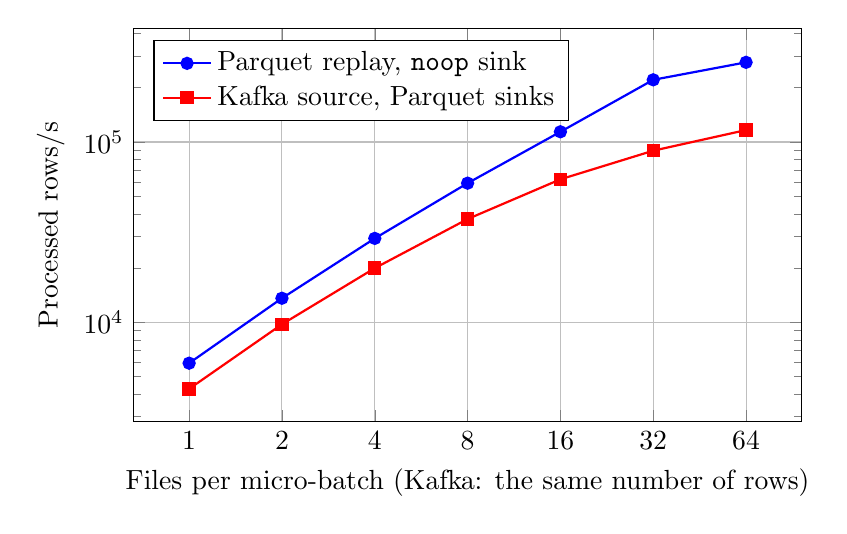
\begin{tikzpicture}
\begin{axis}[
  width=0.70\columnwidth, height=5cm, scale only axis,
  xmode=log, ymode=log, log basis x=2,
  xtick={1,2,4,8,16,32,64}, xticklabels={1,2,4,8,16,32,64},
  xlabel={Files per micro-batch (Kafka: the same number of rows)}, ylabel={Processed rows/s},
  grid=major, legend pos=north west, legend cell align=left,
]
\addplot[mark=*, thick, color=blue, error bars/.cd, y dir=both, y explicit] coordinates {(1,5936) += (0,81) -= (0,90) (2,13605) += (0,251) -= (0,188) (4,29218) += (0,50) -= (0,33) (8,59143) += (0,24) -= (0,17) (16,114009) += (0,1198) -= (0,1511) (32,221381) += (0,1500) -= (0,988) (64,276793) += (0,4661) -= (0,5941)};
\addlegendentry{Parquet replay, \texttt{noop} sink}
\addplot[mark=square*, thick, color=red, error bars/.cd, y dir=both, y explicit] coordinates {(1,4276) += (0,23) -= (0,13) (2,9756) += (0,29) -= (0,46) (4,19983) += (0,45) -= (0,29) (8,37409) += (0,135) -= (0,194) (16,62132) += (0,130) -= (0,238) (32,89549) += (0,474) -= (0,334) (64,116569) += (0,1058) -= (0,736)};
\addlegendentry{Kafka source, Parquet sinks}
\end{axis}
\end{tikzpicture}
\caption{Streaming throughput against micro-batch size from Parquet files and from Kafka (Table~\ref{tab:kafkasweep}); markers give the mean and bars the range of three runs.}
\label{fig:kafkasweep}
\end{figure}
